\documentclass[14pt,a4paper,report]{report}
\usepackage[a4paper, mag=1000, left=2.5cm, right=1cm, top=2cm, bottom=2cm, headsep=0.7cm, footskip=1cm]{geometry}
\usepackage[utf8]{inputenc}
\usepackage[english,russian]{babel}
\usepackage{indentfirst}
\usepackage[dvipsnames]{xcolor}
\usepackage[colorlinks]{hyperref}
\usepackage{listings} 
\usepackage{fancyhdr}
\usepackage{caption}
\usepackage{amsmath}
\usepackage{latexsym}
\usepackage{graphicx}
\usepackage{amsmath}
\hypersetup{
	colorlinks = true,
	linkcolor  = black
}

\usepackage{titlesec}
\titleformat{\chapter}
{\Large\bfseries} % format
{}                % label
{0pt}             % sep
{\huge}           % before-code


\DeclareCaptionFont{white}{\color{white}} 

% Listing description
\usepackage{listings} 
\DeclareCaptionFormat{listing}{\colorbox{gray}{\parbox{\textwidth}{#1#2#3}}}
\captionsetup[lstlisting]{format=listing,labelfont=white,textfont=white}
\lstset{ 
	% Listing settings
	inputencoding = utf8,			
	extendedchars = \true, 
	keepspaces = true, 			  	 % Поддержка кириллицы и пробелов в комментариях
	language = Matlab,            	 	 % Язык программирования (для подсветки)
	basicstyle = \small\sffamily, 	 % Размер и начертание шрифта для подсветки кода
	numbers = left,               	 % Где поставить нумерацию строк (слева\справа)
	numberstyle = \tiny,          	 % Размер шрифта для номеров строк
	stepnumber = 1,               	 % Размер шага между двумя номерами строк
	numbersep = 5pt,              	 % Как далеко отстоят номера строк от подсвечиваемого кода
	backgroundcolor = \color{white}, % Цвет фона подсветки - используем \usepackage{color}
	showspaces = false,           	 % Показывать или нет пробелы специальными отступами
	showstringspaces = false,    	 % Показывать или нет пробелы в строках
	showtabs = false,           	 % Показывать или нет табуляцию в строках
	frame = single,              	 % Рисовать рамку вокруг кода
	tabsize = 2,                  	 % Размер табуляции по умолчанию равен 2 пробелам
	captionpos = t,             	 % Позиция заголовка вверху [t] или внизу [b] 
	breaklines = true,           	 % Автоматически переносить строки (да\нет)
	breakatwhitespace = false,   	 % Переносить строки только если есть пробел
	escapeinside = {\%*}{*)}      	 % Если нужно добавить комментарии в коде
}

\begin{document}

\def\contentsname{Содержание}

% Titlepage
\begin{titlepage}
	\begin{center}
		\textsc{Санкт-Петербургский Политехнический 
			Университет Петра Великого\\[5mm]
			Кафедра компьютерных систем и программных технологий}
		
		\vfill
		
		\textbf{Отчёт по лабораторной работе №2\\[3mm]
			Курс: «Теория автоматического управления»\\[3mm]
			Тема: «Изучение различных форм представления системы»\\[35mm]
			}
	\end{center}
	
	\hfill
	\begin{minipage}{.5\textwidth}
		Выполнил студент:\\[2mm] 
		Бояркин Никита Сергеевич\\
		Группа: 43501/3\\[5mm]
		
		Проверил:\\[2mm] 
		Нестеров Сергей Александрович
	\end{minipage}
	\vfill
	\begin{center}
		Санкт-Петербург\\ \the\year\ г.
	\end{center}
\end{titlepage}

% Contents
\tableofcontents
\clearpage

\chapter{Лабораторная работа №2}

\section{Цель работы}

Получить навыки работы с моделями ВСВ и каноническими представлениями.

\section{Программа работы}

\begin{itemize}
	\item Представить систему в трех канонических формах.
	\item Получить структурные схемы для каждой формы.
	\item Получить матрицы управляемости и матрицы преобразования.
	\item Проверить систему на устойчивость, наблюдаемость и управляемость.
\end{itemize}

\section{Индивидуальное задание}

$
\\
y''+25y'=5u'+25u, y(0)=0, y'(0)=0, u=1(t)\\\\
W(p)=\frac{y}{u}=\frac{5p+25}{p^2+25p}
$

\section{Ход работы}

\subsection{Построение канонических форм}

\subsubsection{Нормальная форма управления}

\begin{equation*}
\text{$W(p)=\frac{5p+25}{p^2+25p}=\frac{y}{u}$}
\end{equation*}

\begin{equation*}
\text{$\frac{y}{5p+25}=\frac{u}{p^2+25p}=x_1$}
\Longrightarrow
\begin{cases}
	\text{$u=x_1(p^2+25p)$} \\
	\text{$y=x_1(5p+25)$}
\end{cases}
\end{equation*}

\begin{equation*}
\begin{cases}
	\text{$px_1=x_2$} \\
	\text{$px_2=u-25x_2$}\\
	\text{$y=25x_1+5x_2$}
\end{cases}
\end{equation*}

\begin{equation*}
\text{$A=$}
\text{$
\begin{bmatrix}
0 & 1 \\
0 & -25 \\
\end{bmatrix}
$}
\text{$, B=$}
\text{$
\begin{bmatrix}
0 \\
1 \\
\end{bmatrix}
$}
\text{$, C=$}
\text{$
\begin{bmatrix}
25 & 5 \\
\end{bmatrix}
$}
\end{equation*}

Проверим корректность полученных матриц $A, B, C$:

\begin{equation*}
\text{$det(A-\lambda)=0$}
\Longrightarrow
\text{$-\lambda(-25-\lambda)=0$}
\Longrightarrow
\begin{cases}
	\text{$\lambda_1=0$} \\
	\text{$\lambda_2=-25$}
\end{cases}
\end{equation*}

Собственные числа совпадают с собственными числами матриц в нормальной форме наблюдения и канонической форме, что свидетельствует о корректности полученных матриц  $A, B, C$.

\begin{equation*}
\text{$W(p)=C(pE-A)^{-1}B=
\begin{bmatrix}
25 & 5 \\
\end{bmatrix}
\begin{bmatrix}
p & -1 \\
0 & p+25\\
\end{bmatrix}^{-1}
\begin{bmatrix}
0 \\
1 \\
\end{bmatrix}=
\begin{bmatrix}
25 & 5 \\
\end{bmatrix}
\begin{bmatrix}
\frac{1}{p} & \frac{1}{p^2+25p} \\
0 & \frac{1}{p+25}\\
\end{bmatrix}
\begin{bmatrix}
0 \\
1 \\
\end{bmatrix}=
$}
\end{equation*}

\begin{equation*}
\text{$=\begin{bmatrix}
	\frac{25(p+25)}{p^2+25p} & \frac{5p+25}{p^2+25p} \\
	\end{bmatrix}\begin{bmatrix}
	0 \\
	1 \\
	\end{bmatrix}=\frac{5p+25}{p^2+25p}
	$}
\end{equation*}

Передаточная функция, полученная в результате преобразования $W(p)=C(pE-A)^{-1}B$, полностью совпадает с исходной, что свидетельствует о корректности полученных матриц  $A, B, C$. 

\begin{figure}[h!]
	\centering
	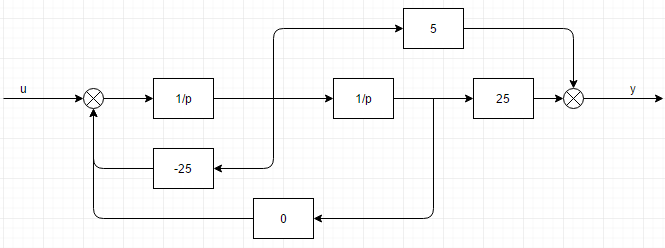
\includegraphics[scale = 0.73]{images/nfu.png}
	\caption{Структурная схема НФУ}
	\label{image:1}
\end{figure}

\subsubsection{Нормальная форма наблюдения}

\begin{equation*}
\text{$W(p)=\frac{5p+25}{p^2+25p}=\frac{y}{u}$}
\Longrightarrow
\text{$(5p+25)u=(p^2+25p)y$}
\Longrightarrow
\end{equation*}

\begin{equation*}
\Longrightarrow
\text{$p^2y+25py-5pu-25u=0$}
\Longrightarrow
\text{$p(p(y)+(25y-5u))+(-25u)=0$}
\end{equation*}

\begin{equation*}
\begin{cases}
	\text{$x_1=py+25y-5u$} \\
	\text{$px_1=25u$} \\
\end{cases}
\Longrightarrow
\begin{cases}
	\text{$x_2=y$}\\
	\text{$x_1=px_2+25x_2-5u$} \\
	\text{$px_1=25u$} \\
\end{cases}
\Longrightarrow
\begin{cases}
	\text{$px_1=25u$} \\
	\text{$px_2=x_1-25x_2+5u$} \\
	\text{$y=x_2$}
\end{cases}
\end{equation*}

\begin{equation*}
\text{$A=$}
\text{$
	\begin{bmatrix}
	0 & 0 \\
	1 & -25 \\
	\end{bmatrix}
	$}
\text{$, B=$}
\text{$
	\begin{bmatrix}
	25 \\
	5 \\
	\end{bmatrix}
	$}
\text{$, C=$}
\text{$
	\begin{bmatrix}
	0 & 1 \\
	\end{bmatrix}
	$}
\end{equation*}

Проверим корректность полученных матриц $A, B, C$:

\begin{equation*}
\text{$det(A-\lambda)=0$}
\Longrightarrow
\text{$-\lambda(-25-\lambda)=0$}
\Longrightarrow
\begin{cases}
	\text{$\lambda_1=0$} \\
	\text{$\lambda_2=-25$}
\end{cases}
\end{equation*}

Собственные числа совпадают с собственными числами матриц в нормальной форме управления и канонической форме, что свидетельствует о корректности полученных матриц  $A, B, C$.

\begin{equation*}
\text{$W(p)=C(pE-A)^{-1}B=
\begin{bmatrix}
0 & 1 \\
\end{bmatrix}
\begin{bmatrix}
p & 0 \\
-1 & p+25\\
\end{bmatrix}^{-1}
\begin{bmatrix}
25 \\
5 \\
\end{bmatrix}=
\begin{bmatrix}
0 & 1 \\
\end{bmatrix}
\begin{bmatrix}
\frac{1}{p} & 0 \\
\frac{1}{p^2+25p} & \frac{1}{p+25}\\
\end{bmatrix}
\begin{bmatrix}
25 \\
5 \\
\end{bmatrix}=
$}
\end{equation*}

\begin{equation*}
\text{$=\begin{bmatrix}
\frac{1}{p^2+25p} & \frac{p}{p^2+25p} \\
\end{bmatrix}\begin{bmatrix}
25 \\
5 \\
\end{bmatrix}=\frac{5p+25}{p^2+25p}
$}
\end{equation*}

Передаточная функция, полученная в результате преобразования $W(p)=C(pE-A)^{-1}B$, полностью совпадает с исходной, что свидетельствует о корректности полученных матриц  $A, B, C$. 

\clearpage

\begin{figure}[h!]
	\centering
	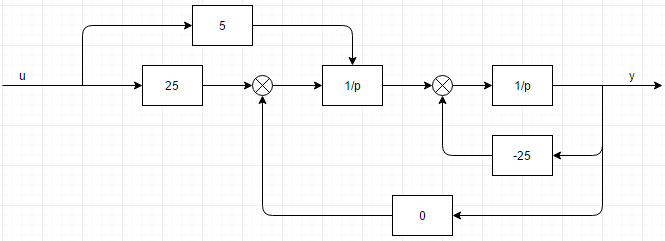
\includegraphics[scale = 0.67]{images/nfn.png}
	\caption{Структурная схема НФН}
	\label{image:2}
\end{figure}

\subsubsection{Каноническая форма}

\begin{equation*}
\text{$W(p)=\frac{5p+25}{p^2+25p}=\frac{5p+25}{p(p+25)}=\frac{1}{p}+\frac{4}{p+25}=\frac{y}{u}$}
\end{equation*}

\begin{equation*}
\begin{cases}
	\text{$\frac{x_1}{u}=\frac{1}{p}$} \\
	\text{$\frac{x_2}{u}=\frac{4}{p+25}$} \\
	\text{$y=x_1+x_2$}
\end{cases}
\Longrightarrow
\begin{cases}
\text{$px_1=u$} \\
\text{$px_2=-25x_2+4u$} \\
\text{$y=x_1+x_2$}
\end{cases}
\end{equation*}

\begin{equation*}
\text{$A=$}
\text{$
	\begin{bmatrix}
	0 & 0 \\
	0 & -25 \\
	\end{bmatrix}
	$}
\text{$, B=$}
\text{$
	\begin{bmatrix}
	1 \\
	4 \\
	\end{bmatrix}
	$}
\text{$, C=$}
\text{$
	\begin{bmatrix}
	1 & 1 \\
	\end{bmatrix}
	$}
\end{equation*}

Проверим корректность полученных матриц $A, B, C$:

\begin{equation*}
\text{$det(A-\lambda)=0$}
\Longrightarrow
	\text{$-\lambda(-25-\lambda)=0$}
\Longrightarrow
\begin{cases}
	\text{$\lambda_1=0$} \\
	\text{$\lambda_2=-25$}
\end{cases}
\end{equation*}

Собственные числа совпадают с собственными числами матриц в нормальной форме управления и нормальной форме наблюдения, что свидетельствует о корректности полученных матриц  $A, B, C$

\begin{equation*}
\text{$W(p)=C(pE-A)^{-1}B=
	\begin{bmatrix}
	1 & 1 \\
	\end{bmatrix}
	\begin{bmatrix}
	p & 0 \\
	0 & p+25\\
	\end{bmatrix}^{-1}
	\begin{bmatrix}
	1 \\
	4 \\
	\end{bmatrix}=
	\begin{bmatrix}
	1 & 1 \\
	\end{bmatrix}
	\begin{bmatrix}
	\frac{1}{p} & 0 \\
	0 & \frac{1}{p+25}\\
	\end{bmatrix}
	\begin{bmatrix}
	1 \\
	4 \\
	\end{bmatrix}=
	$}
\end{equation*}

\begin{equation*}
\text{$=\begin{bmatrix}
	\frac{p+25}{p^2+25p} & \frac{p}{p^2+25p} \\
	\end{bmatrix}\begin{bmatrix}
	1 \\
	4 \\
	\end{bmatrix}=\frac{5p+25}{p^2+25p}
	$}
\end{equation*}

Передаточная функция, полученная в результате преобразования $W(p)=C(pE-A)^{-1}B$, полностью совпадает с исходной, что свидетельствует о корректности полученных матриц  $A, B, C$. 


\begin{figure}[h!]
	\centering
	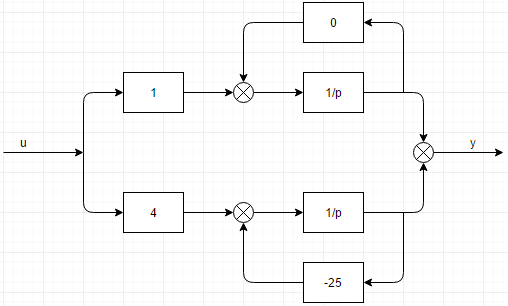
\includegraphics[scale = 0.67]{images/kf.png}
	\caption{Структурная схема КФ}
	\label{image:3}
\end{figure}

\subsection{Преобразования форм}

\subsubsection{Матрицы управляемости}

Матрица управляемости находится как блочная матрица, где первый столбец равен матрице $B$, а второй столбец равен произведению $AB$:

\begin{center}
$U=[B, AB]$
\end{center}

Матрицы управляемости нормальной формы управления (НФУ):

\begin{equation*}
\text{$U=\begin{bmatrix} 0 & 1 \\ 1 & -25 \end{bmatrix}$}
\text{$, U^{-1}=\begin{bmatrix} 25 & 1 \\ 1 & 0 \end{bmatrix}$}
\end{equation*}

Матрицы управляемости нормальной формы наблюдения (НФН):

\begin{equation*}
\text{$U=\begin{bmatrix} 25 & 0 \\ 5 & -100 \end{bmatrix}$}
\text{$, U^{-1}=\frac{1}{500}\begin{bmatrix} 20 & 0 \\ 1 & -5 \end{bmatrix}$}
\end{equation*}

Матрицы управляемости канонической формы (КФ):

\begin{equation*}
\text{$U=\begin{bmatrix} 1 & 0 \\ 4 & -100 \end{bmatrix}$}
\text{$, U^{-1}=\frac{1}{100}\begin{bmatrix} 100 & 0 \\ 4 & -1 \end{bmatrix}$}
\end{equation*}

\subsubsection{Матрицы преобразования}

Матрица преобразования высчитывается по формуле:

\begin{center}
$P=U_{*}U^{-1}$
\end{center}

\begin{itemize}
	\item Матрица преобразования из НФУ в НФН:
	
	\begin{equation*}
	\text{$P=U_{*}U^{-1}=\begin{bmatrix} 25 & 0 \\ 5 & -100 \end{bmatrix}\begin{bmatrix} 25 & 1 \\ 1 & 0 \end{bmatrix}=5\begin{bmatrix} 125 & 5 \\ 5 & 1 \end{bmatrix}$}
	\end{equation*}
	
	Проверим корректность полученной матрицы преобразования $P$. Для этого получим матрицу $B_{*}$ через матрицу $B$. 
	
	\begin{equation*}
	\text{$B_{*}=PB$}
	\Longrightarrow
	\text{$B_{*}=5\begin{bmatrix} 125 & 5 \\ 5 & 1 \end{bmatrix}\begin{bmatrix} 0 \\ 1 \end{bmatrix}=5\begin{bmatrix} 5 \\ 1 \end{bmatrix}=\begin{bmatrix} 25 \\ 5 \end{bmatrix}$}
	\end{equation*}
	
	\item Матрица преобразования из НФУ в КФ:
	
	\begin{equation*}
	\text{$P=U_{*}U^{-1}=\begin{bmatrix} 1 & 0 \\ 4 & -100 \end{bmatrix}\begin{bmatrix} 25 & 1 \\ 1 & 0 \end{bmatrix}=\begin{bmatrix} 25 & 1 \\ 0 & 4 \end{bmatrix}$}
	\end{equation*}
	
	Проверим корректность полученной матрицы преобразования $P$. Для этого получим матрицу $B_{*}$ через матрицу $B$. 
	
	\begin{equation*}
	\text{$B_{*}=PB$}
	\Longrightarrow
	\text{$B_{*}=\begin{bmatrix} 25 & 1 \\ 0 & 4 \end{bmatrix}\begin{bmatrix} 0 \\ 1 \end{bmatrix}=\begin{bmatrix} 1 \\ 4 \end{bmatrix}$}
	\end{equation*}
	
	\item Матрица преобразования из НФН в НФУ:
	
	\begin{equation*}
	\text{$P=U_{*}U^{-1}=\begin{bmatrix} 0 & 1 \\ 1 & -25 \end{bmatrix}\frac{1}{500}\begin{bmatrix} 20 & 0 \\ 1 & -5 \end{bmatrix}=\frac{1}{500}\begin{bmatrix} 1 & -5 \\ -5 & 125 \end{bmatrix}$}
	\end{equation*}
	
	Проверим корректность полученной матрицы преобразования $P$. Для этого получим матрицу $B_{*}$ через матрицу $B$.
	
	\begin{equation*}
	\text{$B_{*}=PB$}
	\Longrightarrow
	\text{$B_{*}=\frac{1}{500}\begin{bmatrix} 1 & -5 \\ -5 & 125 \end{bmatrix}\begin{bmatrix} 25 \\ 5 \end{bmatrix}=\begin{bmatrix} 0 \\ 1 \end{bmatrix}$}
	\end{equation*}
	
	\item Матрица преобразования из НФН в КФ:
	
	\begin{equation*}
	\text{$P=U_{*}U^{-1}=\begin{bmatrix} 1 & 0 \\ 4 & -100 \end{bmatrix}\frac{1}{500}\begin{bmatrix} 20 & 0 \\ 1 & -5 \end{bmatrix}=\frac{1}{25}\begin{bmatrix} 1 & 0 \\ -1 & 25 \end{bmatrix}$}
	\end{equation*}
	
	Проверим корректность полученной матрицы преобразования $P$. Для этого получим матрицу $B_{*}$ через матрицу $B$.
	
	\begin{equation*}
	\text{$B_{*}=PB$}
	\Longrightarrow
	\text{$B_{*}=\frac{1}{25}\begin{bmatrix} 1 & 0 \\ -1 & 25 \end{bmatrix}\begin{bmatrix} 25 \\ 5 \end{bmatrix}=\begin{bmatrix} 1 \\ 4 \end{bmatrix}$}
	\end{equation*}
	
	\item Матрица преобразования из КФ в НФУ:
	
	\begin{equation*}
	\text{$P=U_{*}U^{-1}=\begin{bmatrix} 0 & 1 \\ 1 & -25 \end{bmatrix}\frac{1}{100}\begin{bmatrix} 100 & 0 \\ 4 & -1 \end{bmatrix}=\frac{1}{100}\begin{bmatrix} 4 & -1 \\ 0 & 25 \end{bmatrix}$}
	\end{equation*}
	
	Проверим корректность полученной матрицы преобразования $P$. Для этого получим матрицу $B_{*}$ через матрицу $B$.
	
	\begin{equation*}
	\text{$B_{*}=PB$}
	\Longrightarrow
	\text{$B_{*}=\frac{1}{100}\begin{bmatrix} 4 & -1 \\ 0 & 25 \end{bmatrix}\begin{bmatrix} 1 \\ 4 \end{bmatrix}=\begin{bmatrix} 0 \\ 1 \end{bmatrix}$}
	\end{equation*}
	
	\item Матрица преобразования из КФ в НФН:
	
	\begin{equation*}
	\text{$P=U_{*}U^{-1}=\begin{bmatrix} 25 & 0 \\ 5 & -100 \end{bmatrix}\frac{1}{100}\begin{bmatrix} 100 & 0 \\ 4 & -1 \end{bmatrix}=\begin{bmatrix} 25 & 0 \\ 1 & 1 \end{bmatrix}$}
	\end{equation*}
	
	Проверим корректность полученной матрицы преобразования $P$. Для этого получим матрицу $B_{*}$ через матрицу $B$.
	
	\begin{equation*}
	\text{$B_{*}=PB$}
	\Longrightarrow
	\text{$B_{*}=\begin{bmatrix} 25 & 0 \\ 1 & 1 \end{bmatrix}\begin{bmatrix} 1 \\ 4 \end{bmatrix}=\begin{bmatrix} 25 \\ 5 \end{bmatrix}$}
	\end{equation*}
		
\end{itemize}

\subsection{Характеристики системы}

\subsubsection{Управляемость}

Проверим управляемость системы по критерию Калмана:

\begin{equation*}
\text{$detU=det\begin{bmatrix} 0 & 1 \\ 1 & -25 \end{bmatrix}=-1\neq 0$}
\end{equation*}

Определитель одной из матриц управляемости не нулевой, что означает, что система полностью управляема.

\subsubsection{Наблюдаемость}

Проверим наблюдаемость системы по критерию Калмана:

\begin{equation*}
\text{$N=[C^T,A^TC^T]=[\begin{bmatrix} 25 \\ 5 \end{bmatrix},\begin{bmatrix} 0 & 0 \\ 1 & -25 \end{bmatrix}\begin{bmatrix} 25 \\ 5 \end{bmatrix}]=\begin{bmatrix} 25 & 0 \\ 5 & -100 \end{bmatrix}$}
\end{equation*}

\begin{equation*}
\text{$detN=det\begin{bmatrix} 25 & 0 \\ 5 & -100 \end{bmatrix}=-2505\neq 0$}
\end{equation*}

Определитель одной из матриц наблюдаемости не нулевой, что означает, что система полностью наблюдаема.

\subsubsection{Устойчивость}

По теореме Ляпунова система является устойчивой тогда, когда вещественные части полюсов её передаточной функции отрицательны. В нашем случае полюса передаточной функции равны $p_1=0, p_2=-25$, что означает, что система находится на границе устойчивости. 

\section{Вывод}

Модель ВСВ весьма гибкая, так как помимо трех канонических форм, рассмотренных в работе существуют произвольные формы, которые иногда могут быть полезны. Стоит отметить, что получив матрицы управляемости для модели ВСВ можно легко преобразовать систему, как и к какой либо канонической форме, так и к другому произвольному представлению.

Отличия между каноническими формами наиболее явно проявляются на структурных схемах. Система, представленная в форме управления, имеет два узла суммирования и n узлов размножения. В форме наблюдения - наоборот, два узла размножения и n узлов суммирования. Особенность обеих этих форм - сложные обратные связи между элементами схемы. Альтернатива - форма Лурье, которая требует (n+1) узлов размножения и столько же узлов суммирования. Её преимущество - обратные связи являются более простыми по сравнению с другими вариантами.

В преобразованиях, связанных с матрицами множество мест, в которых легко допустить ошибку, поэтому желательна проверка результата. Самая простая проверка - совпадение собственных чисел матрицы $A$ во всех канонических формах. После этого можно проверить результат, получив передаточную функцию через матрицы $A,B,C$.

В то же время, информация об управляемости, наблюдаемости и устойчивости получается простейшими вычислениями, поэтому эти свойства рекомендуется находить, чтобы получить больше полезной информации о системе.



\end{document}